\subsection{The Straight Line Again}

\begin{tcolorbox}[title=Problem 28, breakable]
    For our purposes here, define two straight 
    lines to be parallel if they have 
    the same slope. Let 
    \[y = ax + b \text{ and } y = cx + d\]
    be the equations of two lines with $b \ne d$.

    (a) If they are parallel, show they they have no point in common.

    (b) If they are not parallel, show theat they have exactly one point in common.
\end{tcolorbox}

\begin{proof}
    Suppose the lines are parallel and do share a comon point.
    Thus $ax + b = cx + d$, but $a = c$ thus $b = d$ which is a contradiction.
\end{proof}

\begin{proof}
    Suppose the lines are not parallel.
    Thus 
    \[
        ax + b = cx + d \iff x(a - c) = d - b \iff x = \frac{d - b}{a - c}.
    \]
    Note since the lines are not parallel \(a \ne c\), thus \(a - c \ne 0\).
    Plugging this back into either equation gives our point of intersection.
\end{proof}

\begin{tcolorbox}[title=Problem 30, breakable]
    If a straight line is expressed in parametric form,
    \[\{P + tA\}_{t \in \mathbb{R}}\]
    and $A = (a_1, a_2)$, what is the slope of the line in terms 
    of the coordinates $A$?
    Does this slope depend on the coordinates of $P$.
\end{tcolorbox}

\textbf{Solution:}
Suppose $P = (p_1, p_2)$. Then 
\[
x = p_1 + t a_1, \quad y = p_2 + t a_2.
\]
The slope of the line is 
\[
\frac{y - p_2}{x - p_1} = \frac{a_2 t}{a_1 t} = \frac{a_2}{a_1}.
\]
Thus the slope does snot depend on the coordinates of $P$.


\subsection{The Parabola}

\begin{tcolorbox}[title=Problem 5, breakable]
    Sketch the graph $x^2 +  y^2 - 4x + 2y - 20 = 0$.
\end{tcolorbox}

\textbf{Solution:} $x^2 + y^2 - 4x + 2y - 20 = (x^2 - 4x) + (y^2 + 2y) - 20.$  
Completing the square on $x$ gives $x^2 - 4x = (x-2)^2 - 4$,  
and completing the square on $y$ gives $y^2 + 2y = (y+1)^2 - 1$.  
Thus 
\[(x-2)^2 - 4 + (y+1)^2 - 1 - 20 = 0 \implies (x-2)^2 + (y+1)^2 = 25\]
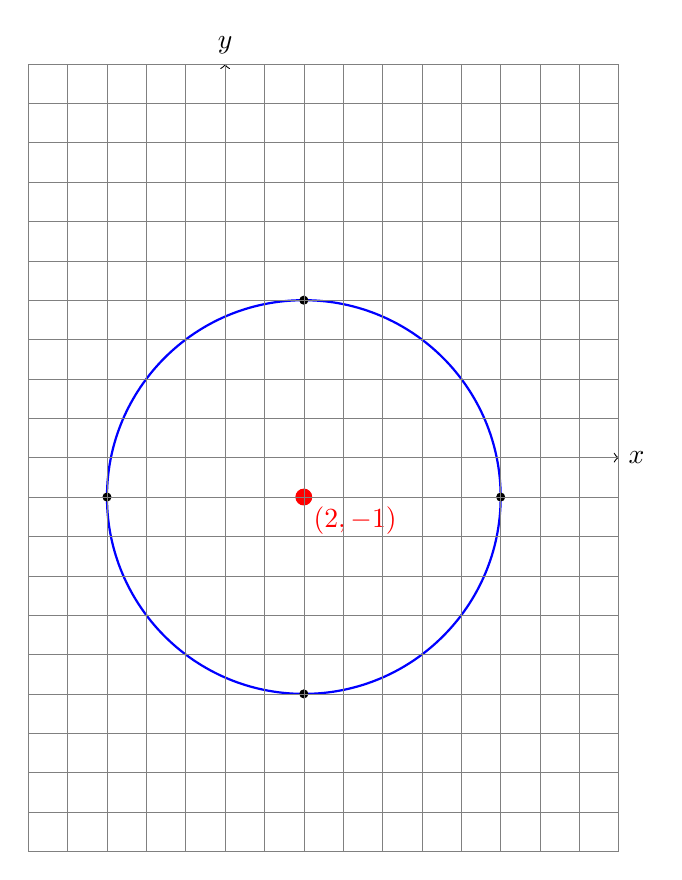
\begin{tikzpicture}[scale=0.5]
    % Draw axes
    \draw[->] (-5,0) -- (10,0) node[right] {$x$};
    \draw[->] (0,-10) -- (0,10) node[above] {$y$};
    
    % Draw the circle
    \draw[blue, thick] (2,-1) circle [radius=5];
    
    % Mark the center
    \filldraw[red] (2,-1) circle (0.2) node[below right] {$(2,-1)$};
    
    % Optional: mark radius points
    \filldraw[black] (2+5,-1) circle (0.1) node[below right] {};
    \filldraw[black] (2-5,-1) circle (0.1) node[below left] {};
    \filldraw[black] (2,-1+5) circle (0.1) node[above left] {};
    \filldraw[black] (2,-1-5) circle (0.1) node[below left] {};
    
    % Optional: grid
    \draw[very thin, gray] (-5,-10) grid[step=1] (10,10);
\end{tikzpicture}

\subsection{The Ellipse}

\begin{tcolorbox}[title=Problem 1, breakable]
    Sketch the graph of the following equations.
    In each case, indicate the center of the ellipse,
    and its extremities.
    \[\frac{x^2}{16} + \frac{y^2}{4} = 1\]
\end{tcolorbox}

\textbf{Solution:} Center is $(0, 0)$.
Extremities are $(\pm 4, 0)$ and $(0, \pm 2)$.
\begin{figure}[h!]
    \centering
    \includegraphics[width=0.5\textwidth]{images/ellipse_again.png}
\end{figure}

\subsection{The Hyperbola}

\begin{tcolorbox}[title=Problem 8, breakable]
    Sketch the graphs of the following curves, defined by the 
    given equations.

    $xy = 4$.
\end{tcolorbox}

\begin{figure}[h!]
    \centering
    \includegraphics[width=0.5\textwidth]{images/hyperbola.png}
\end{figure}

\subsection{Rotation of Hyperbolas}

\begin{tcolorbox}[title=Problem 2, breakable]
    Rotate the hyperbola $H$ defined by the equation $xy = 1$
    by $-\pi/4$. What is the equation satisfied by the image of $H$.
\end{tcolorbox}
\[v^2 - u^2 = 2\]

\begin{tcolorbox}[title=Problem 8, breakable]
    Prove the statement made in the text: If $G$ is rotation 
        and $F_r$ is a dilation by $r$, $G \circ F = F \circ G$.
\end{tcolorbox}

\begin{proof}
    Let $P = (x, y)$ be an arbitrary point.
    A dilation by $r$ is
    \[
    F_r(P) = r \begin{bmatrix} x \\ y \end{bmatrix},
    \]
    and a rotation by angle $\theta$ is 
    \[
    G(P) = \begin{bmatrix} \cos\theta & -\sin\theta \\ \sin\theta & \cos\theta \end{bmatrix} \begin{bmatrix} x \\ y \end{bmatrix}.
    \]
    Then
    \[
    G(F_r(P)) 
    = \begin{bmatrix} \cos\theta & -\sin\theta \\ \sin\theta & \cos\theta \end{bmatrix} \left( r \begin{bmatrix} x \\ y \end{bmatrix} \right)
    = r \begin{bmatrix} \cos\theta & -\sin\theta \\ \sin\theta & \cos\theta \end{bmatrix} \begin{bmatrix} x \\ y \end{bmatrix}.
    \]
    Similarly,
    \[
    F_r(G(P)) 
    = r \left( \begin{bmatrix} \cos\theta & -\sin\theta \\ \sin\theta & \cos\theta \end{bmatrix} \begin{bmatrix} x \\ y \end{bmatrix} \right)
    = r \begin{bmatrix} \cos\theta & -\sin\theta \\ \sin\theta & \cos\theta \end{bmatrix} \begin{bmatrix} x \\ y \end{bmatrix}.
    \]
\end{proof}